\chapter{Btlejuice and Gattacker}
\label{chapter5}
\thispagestyle{empty}

\noindent 
Man-In-The-Middle attacks are probably the most interesting cases on which to work on, even though they are much harder to accomplish than what theoretical concepts may lead to think.

The main target of the attack is to connect to the device, extract its informations and features, MAC address included, and create copy, a dummy device. The attacker then waits for legit user to connect, and forwards the messages to the destination. In order to accomplish the attack, it is mandatory to take into account the Bluetooth range and thus be close to the target device.

Devices and tools as Ubertooth or Adafruit Bluefruit sniffer provide Man-In-The-Middle support, but they are quite expensive solutions. We choose to use two open-source tools, \texttt{btlejuice} and \texttt{gattacker}, which can be downloaded freely from their Github repositories. These two tools are independently built, but accomplish the same goal of providing proof-of-concept MITM functionalities. As usual in the security field, it should be considered that real hacking (or tampering without permission) can lead to undesired consequences.

\section{Btlejuice}
Btlejuice is a complete framework based on Node.js that includes an interception core, an interception proxy, a dedicated web interface as well as Python and Node.js bindings.
The requirement for this tool are the Bluetooth and Bluez suites and their respective libraries, as well as Node.js (>=4.3.2) and \texttt{npm}. The installation process is not as easy as it seems, since there are numerous dependencies to satisfy. Explanations and tutorials are available on Btlejuice official Github page \cite{btlejuice-repo}.

Up to the current version, Btlejuice is able to provide support for Bluez 5.x and JustWorks BLE devices, while other connectivity types may not work.

\begin{figure}
	\centering
	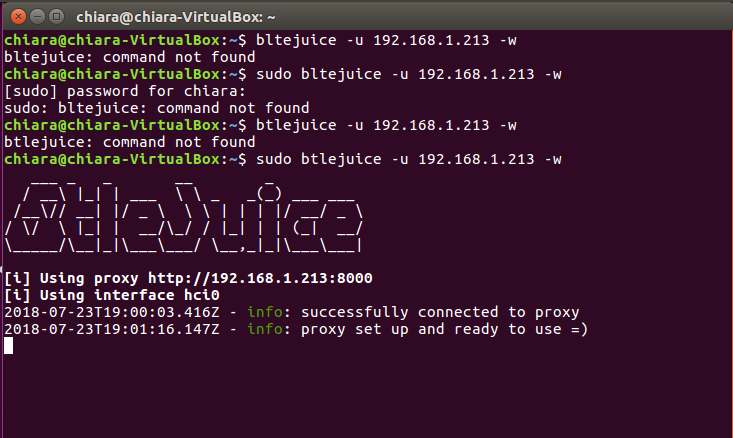
\includegraphics[width=0.8\textwidth]{host1.png}
	\caption{Host Pov - Establishing the Connection with the proxy.}
	\label{fig:btlejuice-host1}
\end{figure}

\begin{figure}
	\centering
	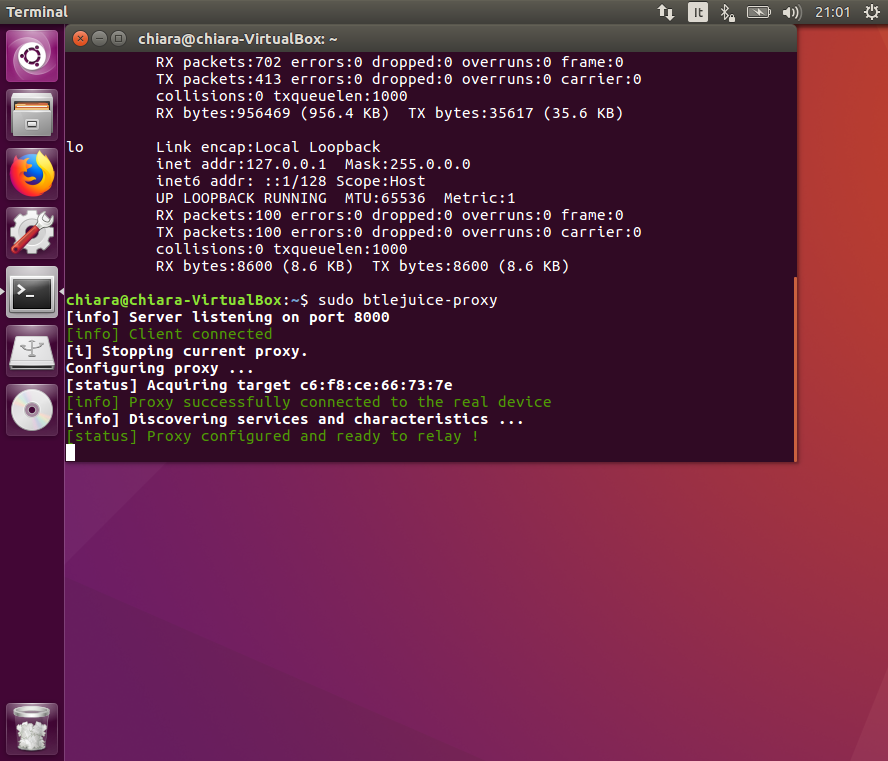
\includegraphics[width=0.8\textwidth]{proxy1.png}
	\caption{Proxy POV - Establishing the Connection with the host and copying the services of the device}
	\label{fig:btlejuice-proxy1}
\end{figure}

\begin{figure}
	\centering
	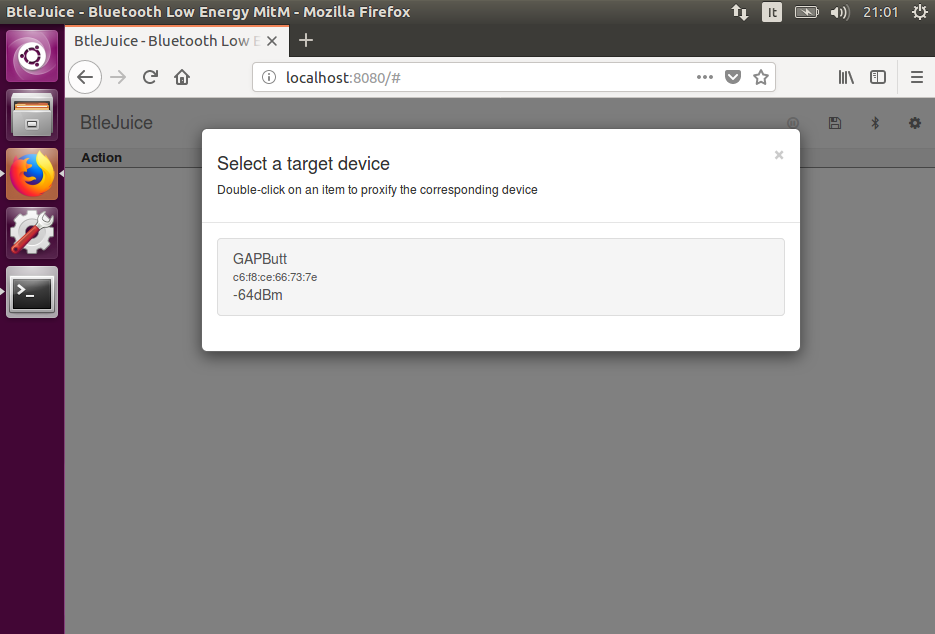
\includegraphics[width=0.8\textwidth]{host2.png}
	\caption{Host Pov - Btlejuice UI}
	\label{fig:btlejuice-host2}
\end{figure}

In order to use Btlejuice it is necessary to install \texttt{Noble} on the host machine and \texttt{Bleno} on the proxy. They are two external Node.js modules that model the Central and Peripheral device, and are necessary to rebuild the connection structure.

Btlejuice main freatures are the live GATT operations and data sniffing; it also allows on-the-fly data manipulation and creation of a copy of the device while being connected to it, using CSR adapters. This tool has, on the other hand, some limitations: Noble doesn't support long writes and there is some latency due to the connection from BLE to websocket and then back to BLE. Other issues may arise when the device keep connections or advertises during a short delay. In conclusion, Btlejuice is very promising and has indeed some strong features, but there is the need for more testing and debugging.

\section{Gattacker}
Gattacker \cite{gattacker-repo} is another interesting and powerful instrument for Man-In-The-Middle attacks, presenting also additional complexity with respect to Btlejuice. \texttt{gatttacker} installation procedure is quite similar to the previous one as it requires node and \texttt{npm}, together with Bluetooth and Bluez dependencies.

The deployment concept is basically the same: as it recreates the connection between two devices it needs to run on two separate machines. Testing sessions demonstrate that it is impossible to use it without a Virtrual Machine, as the program needs more than one Bluetooth interface. The two Virtual Machines will work as \textit{master} and \textit{slave} devices, respectively using the modules of Noble and Bleno. We also found that it is possible to run them on separate physical machines, as long as the \textit{master} device knows the IP address of the \textit{slave} in its configuration file.

Once operating, the two platforms run in parallel in order to clone the device and create a dummy.
There is a strict sequences of steps to follow in order to perform the attacks, and inaccurate executions may lead up to unsuccessful attempts. Particular care must be put also towards the target device, which must not be paired at the moment of the attack. This is necessary as it will be advertising its characteristics and services on the main channel: in the first steps, the master device simply listens to advertisement packets and creates an internal structure of \texttt{json} documents to describe it accurately; later, this same structure will be used to clone the device and trick the user into connecting with it. In Listing \ref{list:gattacker} we can see the commands which summarize this procedure.
\lstinputlisting[caption={\texttt{gattacker}'s initial commands to start a MITM attack},label={list:gattacker},language=bash]{GATTacker-cmd.sh}

We tested this tool in two different settings: the first time, we tried to perform an attack on the Magic Blue smart bulb, while the second time we flashed a program on the STM IoT node and performed the attack on that. We reported our findings, limited to the STM board, in Appendix \ref{appendixC}.

Gattacker has a support to replay actions: they can be stored in log files and then replayed when necessary, also from the BLESniffer mobile app.

In conclusion, we can say that \texttt{gattacker} is less intuitive to use than \texttt{btlejuice}, and also in this case some more testing is needed.